\documentclass[xcolor=pdftex,dvipsnames,table,mathserif,aspectratio=169]{beamer}
\usetheme{metropolis}

%\usetheme{Darmstadt}
%\usepackage{times}
%\usefonttheme{structurebold}

\usepackage[english]{babel}
%\usepackage[table]{xcolor}
\usepackage{pgf,pgfarrows,pgfnodes,pgfautomata,pgfheaps}
\usepackage{amsmath,amssymb,setspace,centernot}
\usepackage[latin1]{inputenc}
\usepackage[T1]{fontenc}
\usepackage{relsize}
\usepackage{stmaryrd}
\usepackage{pdfpages}
\usepackage{booktabs}
\usepackage[absolute,overlay]{textpos} 


\newenvironment{reference}[2]{% 
  \begin{textblock*}{\textwidth}(#1,#2) 
      \footnotesize\it\bgroup\color{red!50!black}}{\egroup\end{textblock*}} 

\DeclareMathSizes{10}{10}{6}{6} 
\AtBeginSection[]{
  \begin{frame}
  \vfill
  \centering
  \begin{beamercolorbox}[sep=8pt,center,shadow=true,rounded=true]{title}
    \usebeamerfont{title}\insertsectionhead\par%
  \end{beamercolorbox}
  \vfill
  \end{frame}
}
\begin{document}
\title{Conduct}
\author{Chris Conlon}
\institute{Grad IO}
\date{\today}

\frame{\titlepage}

\begin{frame}{Conduct Overview}
\begin{itemize}
\item A second set of important questions in IO is being able to use data to decide whether firms are \alert{competing} or \alert{colluding}.
\item Absent additional restrictions, we cannot generally look at data on $(P,Q)$ and decide whether or not collusion is taking place.
\item We can make progress in two ways: (1) parametric restrictions on marginal costs; (2) exclusion restrictions on supply.
\begin{itemize}
\item Most of the literature focuses on (1) by assuming something like: $\ln mc_{jt} = x_{jt} \gamma_1 + w_{jt} \gamma_2 + \omega_{jt}$.
\item In principle (2) is possible if we have instruments that shift demand for products but not supply. (These are much easier to come up with than ``supply shifters'').
\end{itemize}
\end{itemize}
\end{frame}

\begin{frame}{A famous plot (Bresnahan 87)}
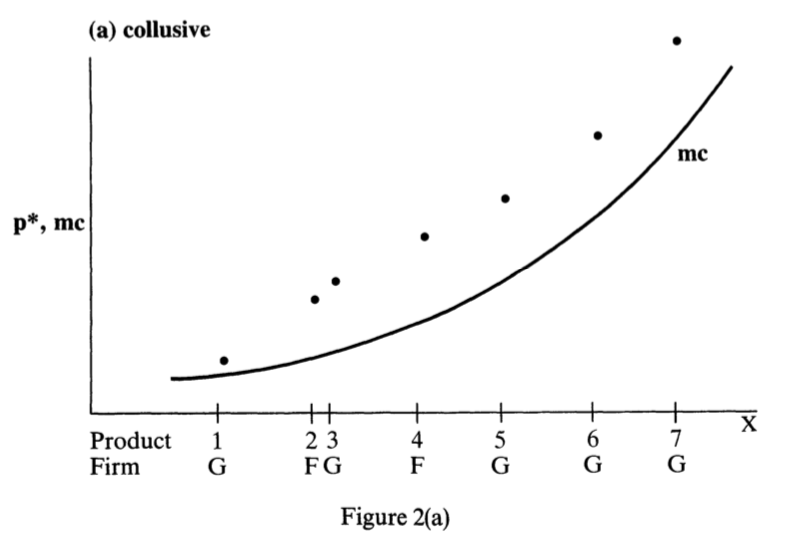
\includegraphics[width = 6.6cm]{./resources/bres_plot1.png}
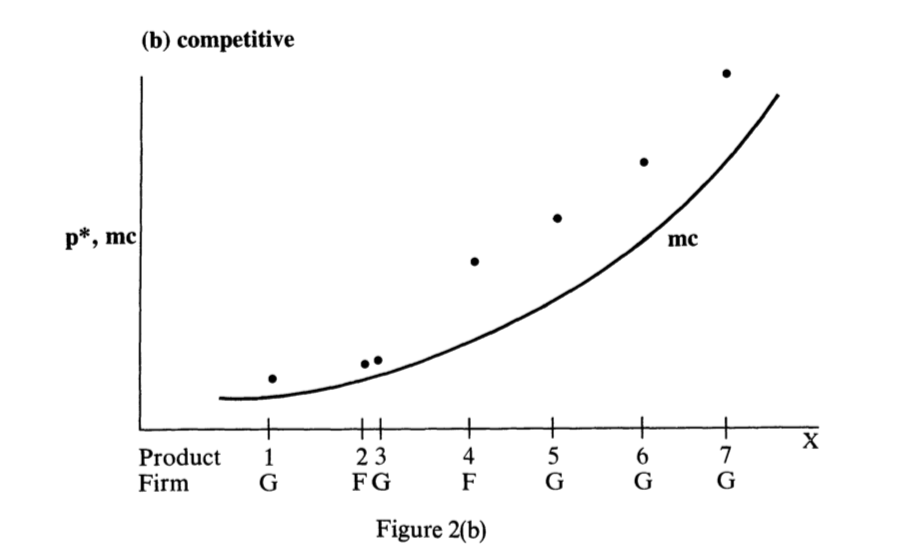
\includegraphics[width = 6.9cm]{./resources/bres_plot2.png}
\end{frame}



\begin{frame}{Testing For Conduct: Challenges}
\begin{itemize}
\item Recall the $\Delta$ matrix which we can write as $\Delta=\tilde{\Delta}\, \odot A$, where $\odot$ is the element-wise or Hadamard product of two matrices. 
\begin{itemize}
\item $\tilde{\Delta}$ is the matrix of demand derivatives with $\Delta{(j,k)} = \frac{\partial q_j}{\partial p_k}$ for all elements.
\item $A_{(j,k)} =1$ if $(j,k)$ have the same owner and $0$ otherwise.
\end{itemize}
\item Mergers are about changing $0$'s to $1$'s in the $A$ matrix.
\item Matrix form of FOC: $q(\mathbf{p}) = \Omega(\mathbf{p})\cdot(\mathbf{p}-\mathbf{mc})$
\end{itemize}
\end{frame}

\begin{frame}
\frametitle{Testing For Collusion: Challenges}
We derived those conditions from multi-product Bertrand FOCs:
\begin{eqnarray*}
\arg \max_{p \in \mathcal{J}_f} \pi_f (\mathbf{p}) &=& \sum_{j \in \mathcal{J}_f} (p_j - c_j) \cdot q_j(\mathbf{p}) +  \alert{\kappa_{fg} \sum_{j \in \mathcal{J}_g} (p_j - c_j) \cdot q_j(\mathbf{p})} \\
\rightarrow 0&=& q_j(\mathbf{p}) + \sum_{k \in (\mathcal{J}_f,\mathcal{J}_g)} \alert{\kappa_{fg}}\cdot (p_k - c_k) \frac{\partial q_{k}}{\partial p_j}(\mathbf{p}) 
\end{eqnarray*}
\begin{itemize}
\item Now we have generalized the $A(\kappa)$ matrix.
\item Instead of $0$'s and $1$'s we now have $\kappa_{fg} \in [0,1]$ representing how much firm $f$ cares about the profits of $g$.
\begin{itemize}
\item If $f$ and $g$ merge (or fully colluded) then $\kappa_{fg} =1$
\item Often in the real world firms cannot reach fully collusive profits and $\kappa_{fg} \in (0,1)$.
\item Evidence that $\kappa_{fg} > 0$ is not necessarily evidence of malfeasance, just a deviation from \alert{static Bertrand pricing}.
\end{itemize}
\end{itemize}
\end{frame}

\begin{frame}
\frametitle{Reasons for Deviations from Static Bertrand}
\small
\begin{description}
\item[Biased estimates of own and cross price derivatives:] For anything to work, you have correct estimates of $\tilde{\Omega}$. My prior is most papers \alert{underestimate} cross price elasticites.
\item[Vertical Relationships:] Who sets supermarket prices? Just the retailer? Just the manufacturer? Some combination of both? Retailers tend to \alert{soften} downstream price competition.
\item[Faulty Timing Assumptions:] Bertrand is a simultaneous move pricing game. Lots of alternatives (Stackelberg leader-follower, Edgeworth cycles, etc.).
\item[Dynamics and Dynamic Pricing:] Forward looking firms or consumers might not set static Nash prices. [e.g. Temporary Sales, Switching Costs, Network Effects, etc.]
\item[Unmodeled Supergame:] Maybe firms are legally tacitly colluding, higher prices might be about what firms believe will happen in a price war.
\end{description}
\end{frame}



\begin{frame}
\frametitle{Algorithm \#1: Bertrand Deviations}

\begin{itemize}
\item Recover $\tilde{\Omega}$ from demand alone.
\item Recover marginal costs $\widehat{\mathbf{mc}} = \mathbf{p} +(O.*\tilde{\Omega}(\mathbf{p}))^{-1} q(\mathbf{p})$.
\end{itemize}
Challenges:
\begin{itemize}
\item Given $[\mathbf{q},\mathbf{p},\tilde{\Omega},O]$ I can always produce a vector of marginal costs $\mathbf{c}$ that rationalizes what we observe. [ie: $J$ equations $J$ unknowns].
\item Maybe some vectors of $\mathbf{c}$ look less ``reasonable'' than others.
\begin{itemize}
\item ie: I have a parametric model of MC in mind. 
\item Can test that model with GMM objective of $c_{jt}$ on regressors.
\item Maybe marginal costs cannot deviate too much within product from period to period.
\item Marginal costs $\leq 0$ seem problematic. [Might just be that your estimates for demand are too inelastic...]
\end{itemize}
\end{itemize}
\end{frame}

\begin{frame}
\frametitle{Algorithm \#2: Simultaneous Supply and Demand}
\begin{itemize}
\item Recover $\tilde{\Omega}$ from demand and parametric assumption on supply (GMM with both sets of moments).
\item I can impose $c > 0$ by using $\ln mc_{jt} = x_{jt} \gamma_1 + w_{jt} \gamma_2 + \omega_{jt}$.
\item The fit of my supply side will also inform my demand parameters, particularly $\alpha$ the price coefficient. [BLP 95 used this for additional power with lots of random coefficients and potentially weak instruments].
\end{itemize}
Challenges:
\begin{itemize}
\item Am I testing conduct? Or am I testing the linear functional form for my supply model?
\item Will a missing $z_{jt}$ change whether or not I believe firms are colluding?
\end{itemize}
\end{frame}



\begin{frame}{\normalsize Algorithm \#3: Exclusion Restrictions}
\small
\begin{itemize}
\item We provide a formal test for four alternative models of conduct based on the exclusion restriction test in Berry and Haile (2014) 
\begin{eqnarray*}
\widehat{mc_{jt}}(\kappa,\hat{\theta}) &=& \lambda_j +  \gamma_1 x_{jt} + \gamma_2 w_{jt} + \omega_{jt}\\
\omega_{jt} &=& \widehat{mc_{jt}}(\kappa,\hat{\theta}) - \lambda_j -  \gamma_1 x_{jt} - \gamma_2 w_{jt} \\
0 &=& E[ \omega_{jt} | \lambda_j, x_{jt}, w_{jt}, \alert{z_{jt}^s}]
\end{eqnarray*}
\item $w_{jt}$: cost shifters (price of corn for Corn Flakes, price of rice for Rice Krispies).
\item $z_{jt}^s$: should \alert{not} shift marginal costs under the true model of conduct but could potentially shift marginal costs under the alternative. A good choice is \alert{markup shifters}.
\begin{itemize}
\item BLP instruments
\item Cost shifters for other products (Price of Rice for Corn Flakes, Price of Corn for Rice Krispies).
\item $\kappa$ parameters or $\kappa$ weighted diversion.
\end{itemize}
\end{itemize}
\end{frame}

\begin{frame}{Start with BLP(95/99) / Nevo (2001)}
Utility of consumer $i$ for product $j$ and store-week $t$ as:
\begin{align*}
    u_{ijt} = \delta_{jt}+ \mu_{ijt}+  \epsilon_{ijt}
\end{align*}
Market shares are given by:
\begin{align*}
    s_{jt}(\delta_{\cdot t},\theta_2) = \int \frac{\exp[ \delta_{jt} + \mu_{ijt} ]}{\sum_{k \in J_t} \exp[ \delta_{kt} + \mu_{ikt} ]} f(\mu_{it} \mid \widetilde{\theta}_2) \, d\mu_{it}.
\end{align*}
BH2014 show that one can invert the vector of observed market shares $\mathcal{S}_t$ to solve for $\delta_{t}=D_{t}^{-1}(\mathcal{S}_t, \theta_2)$.\\
\end{frame}

\begin{frame}[plain]
\frametitle{Supply Side}
Consider the multi-product Bertrand FOCs:
\footnotesize
{\begin{eqnarray*}
\arg \max_{p \in \mathcal{J}_f} \pi_f (\mathbf{p}) &=& \sum_{j \in \mathcal{J}_f} (p_j - c_j) \cdot s_j(\mathbf{p}) +  \kappa_{fg}\sum_{k \in \mathcal{J}_g} (p_k - c_k) \cdot s_k(\mathbf{p}) \\
0&=& s_j(\mathbf{p}) + \sum_{k \in \mathcal{J}_f} (p_k - c_k) \frac{\partial s_{k}}{\partial p_j}(\mathbf{p}) + \sum_g  \alert{\kappa_{fg} \sum_{l \in \mathcal{J}_g} (p_l - c_l) \frac{\partial s_{l}}{\partial p_j}(\mathbf{p})}\\
\end{eqnarray*}
}
It is helpful to define the matrix $\Omega_{(j,k)}(\mathbf{p})  = - \frac{\partial s_{j}}{\partial p_k}(\mathbf{p})$:
\begin{eqnarray*}
A(\kappa)_{(j,k)} = \left\{\begin{array}{lr}
          1 & \text{for }  j \in \mathcal{J}_f \\ 
       	  \kappa_{fg} & \text{for }  j \in \mathcal{J}_f, k \in \mathcal{J}_g\\
	  0 & \text{o.w}\\
        \end{array} \right\}
\end{eqnarray*}
We can re-write the FOC in matrix form:
\begin{eqnarray*}
        s(\mathbf{p}) &= (A(\kappa) \odot \Omega(\mathbf{p})) \cdot (\mathbf{p} - \mathbf{mc}), \\
       \mathbf{mc} &=  \mathbf{p} - \underbrace{(A(\kappa) \odot \Omega(\mathbf{p}))^{-1} s(\mathbf{p})}_{\eta(\mathbf{p},\mathbf{s},\theta_2,\kappa)}.
\end{eqnarray*}
\end{frame}

\begin{frame}{Simultaneous Problem}
Assume additivity, and write in terms of structural errors:
\begin{align*}
\xi_{jt} &=\delta_{jt}(\mathcal{S}_t,\widetilde{\theta}_2) - \theta_1[x_{jt}, \, \alert{v_{jt}}] - \alpha p_{jt} \\
\omega_{jt} &= f \left( p_{jt} - \eta_{jt}(\mathbf{p},\mathbf{s},\theta_2,\kappa) \right) - h(x_{jt}, \alert{w_{jt}},\theta_3)
\end{align*}
We've highlighted the two \alert{exclusion restrictions}:
\begin{itemize}
\item Cost shifters $w_{jt}$
\item Demand shifters $v_{jt}$
\end{itemize}
To simplify slides we let $f(x)=x$ (often $f(x) =\log(x))$.
\end{frame}

\begin{frame}{Simultaneous Problem: Menu Approach}
Assume two models of conduct (correct: $\kappa_0$) (incorrect: $\kappa_1$)
\begin{align*}
%\label{eq:both_mc}
f(p_{jt} -\eta_{jt}(\kappa_0))= h(x_{jt},w_{jt};\theta_3^0)+  \omega_{jt}^{0},\\
f(p_{jt} -\eta_{jt}(\kappa_1))= h(x_{jt},w_{jt};\theta_3^1)+  \omega_{jt}^{1}.
\end{align*}
Write things in terms of the markup difference:
\begin{align*}
p_{jt} -\eta_{jt}(\kappa_1)= h(x_{jt},w_{jt};\theta_3)+ \overbrace{\lambda \cdot  \Delta \eta_{jt}(\mathbf{p},\mathbf{s},\theta,\kappa_0,\kappa_1) +   \omega_{jt}}^{\widetilde{\omega_{jt}}}
\end{align*}
Tempting idea: run the above regression and test if $\lambda=0$.
\begin{itemize}
\item True model $\lambda=0$, alternate model $\lambda \neq 0$. \pause
\item $\eta_{jt}$ is \alert{endogenous}: it depends on everything including $(\xi,\omega)$.
\end{itemize}
\end{frame}


\begin{frame}{An Old Problem}
\begin{itemize}
\item Bresnahan (1980/1982) recognized this problem: we need ``rotations of demand''.
\item Most of the literature followed Bresnahan (1987):
\begin{itemize}
\item $\omega_{jt}$ is \alert{measurement error in price} 
\item Ex: Bonnet and Dubois (2010) $E[\ln(\omega_{jt}) | x_{jt},w_{jt}]=0$:
\begin{align*}
\log(p_{jt} -\eta_{jt}(\kappa,\widehat{\theta}_2))) = h(x_{jt},w_{jt},\theta_3) + \ln \omega_{jt}
\end{align*}
\end{itemize}
\item Other idea: put markup back on RHS and test $\lambda=1$
\begin{align*}
p_{jt} = h(x_{jt},w_{jt},\theta_3)+ \lambda\cdot  \eta_{jt}(\kappa,\widehat{\theta}_2)+ \omega_{jt}
\end{align*}
\begin{itemize}
\item ``Informal'' test of Villas Boas (2007): $E[\omega_{jt} | x_{jt},w_{jt}]=0$.
\item Pakes (2017) uses Wollman (2018) data and BLP IV $E[\omega_{jt} | x_{jt},w_{jt},f(x_{-j})]=0$.
\end{itemize}
\end{itemize}
\end{frame}

\begin{frame}{A subtle solution}
\begin{itemize}
\item Berry Haile 2014 tell us we need \alert{marginal revenue shifters} to act as \alert{exclusion restrictions}.
\item We need an instrument for $\Delta \eta_{jt}(\mathbf{p},\mathbf{s},\theta,\kappa_0,\kappa_1)$
\begin{itemize}
\item Maybe not so hard since it is basically a function of everything.
\item Cannot have a direct effect on $mc_{jt}$ (exclusion restriction).
\end{itemize}
\item Idea would be to use $E[\omega_{jt} | x_{jt}, w_{jt}, z_{jt}^S]=0$:
\begin{align*}
 p_{jt} - \eta_{jt}(\mathbf{p},\mathbf{s},\theta_2,\kappa)  =  h(x_{jt}, w_{jt},\theta_3)  + \omega_{jt} 
\end{align*}
\end{itemize}
\end{frame}

\begin{frame}{Candidate Instruments for $z_{jt}^s$}
\begin{enumerate}
\item The demand shifter $v_{jt}$: maybe easy to find??
\begin{itemize}
\item We use product recalls; prices of complements don't work so well.
\end{itemize}
\item BLP instruments $f(x_{-j})$: not always strong
\begin{itemize}
\item Amit and JF have a nice paper showing how to choose $f(x_{-j})$
\end{itemize}
\item Can use the same logic to construct $v_{-jt}$ or $w_{-jt}$
\begin{itemize}
\item ie: cost shifters (or demand shifters) of competing goods.
\item Price of rice for Corn Flakes; price of corn for Rice Krispies.
\item Will depend on closeness of substitutes $\Delta PPI$ or $D_{jk}$.
\end{itemize}
\item Observed Conduct Shifters: $\kappa_{fg}$
\begin{itemize}
\item Usually conduct is \alert{unobserved} if we are testing it!
\item Index Inclusion Events (Fiona, Kennedy et. al); BlackRock-BGI Acquisition (AST)
\item Miller Weinberg (2017) use (pre/post merger for cartel participants).
\end{itemize}
\end{enumerate}
\end{frame}

\begin{frame}{Things that don't work}
\begin{itemize}
\item $\xi_{jt}$ only makes sense if you believe $Cov(\xi_{jt},\omega_{jt})=0$.
\item $p_{j,t,-s}$ (Hausman instruments) same good in other markets: pick up cost shocks (but could pick up changes in conduct!). 
\item If it isn't in one of our equations: does it have anything to do with demand or supply?
\item It turns out that 2SLS analog $E[\Delta \eta_{jt} | x_t, w_t, v_t,Z_{jt}^e]=\widehat{\Delta \eta_{jt}}$ doesn't add much:
\begin{itemize}
\item Markups aren't a linear function of observables.
\item Coefficients are (probably) quite different across products.
\end{itemize}
\end{itemize}
\end{frame}













\end{document}